\chapter{Requirements and Technological Context}

As discussed in in the introduction \ref{sec:scope}, the main aim is the development of a VS Code Language extension that operates on par with
well-established tooling for other programming languages. The following requirements define the expected capabilities and characteristics the extension must demonstrate.

\begin{multicols}{2}
  \subsection*{Functional Requirements}
  \begin{enumerate}
    \item The extension must provide syntax highlighting for the target language, differentiating keywords, operators, literals, and identifiers.
    \item The extension must provide basic code completion suggestions based on language keywords and the abstract syntax tree (AST) generated by Langium.
    \item The extension must be able to validate data types within the language, providing warnings or errors when type mismatches occur.
    \item The extension must perform semantic analyses to detect invalid constructs, undefined variables, and other semantic errors.
    \item The extension must display syntax and semantic error messages in the editor in real-time as the user edits the code.
    \item The extension must utilize the Langium framework for language specification, parser generation, and language service implementation.
  \end{enumerate}

  \columnbreak

  \subsection*{Non-Functional Requirements}
  \begin{enumerate}
    \item The extension must respond to user edits with syntax and semantic feedback within 100-250ms for files of average size.
    \item The extension must provide a user-friendly experience that is consistent with other popular VS Code extensions.
    \item The extension must be structured and commented in a way that allows future developers to understand and extend its functionality easily.
    \item The extension must be compatible with the latest version of Visual Studio Code at the time of its release and be developed using Langium, with consideration for future maintenance and version support.
    \item The extension must be able to handle files of immense size (around 10000 lines) of code within the bounds of 1 second.
    \item The extension must be delivered with clear and comprehensive documentation, including installation, usage, and extension of its features.
  \end{enumerate}
\end{multicols}

\section{Alternative Technologies}

This extension is implemented using \textbf{Langium}, which itself builds upon the standardized \textbf{Language Server Protocol (LSP)}~\cite{LSP}, yet
there are several other technologies and approaches available for creating Visual Studio Code language extensions. At its core, the LSP allows tooling for programming
languages to be developed in a modular, editor-independent manner, making it possible to implement a language server in any language that can communicate via JSON-RPC.

One common approach is to implement a language server using general-purpose programming languages (e.g., TypeScript, Java, or Rust) combined with parser generation libraries.
Technologies such as \textbf{Jison}~\cite{Jison}, \textbf{Nearley}~\cite{Nearley}, and \textbf{PEG.js}~\cite{PEGjs} offer a range of options for specifying a language's grammar
and creating a parser. These libraries vary in design and capabilities and may need extra components, such as dedicated lexers and scoping to enable fully-fletched tooling.

In contrast, more comprehensive technologies such as \textbf{ANTLR}~\cite{ANTLR} and \textbf{Langium} go beyond
basic parsing. ANTLR provides a mature and highly optimized lexer and parser generation framework that is widely used across many programming languages, while Langium offers
an end-to-end solution for language engineering - including built-in support for scoping, indexing, and validation - making it especially suited for creating fully
featured language servers.

For basic syntax highlighting and lexical analysis, \textbf{TextMate}-style grammars~\cite{TextMate} can be used, offering a lightweight approach when deep semantic understanding is not required.
Meanwhile, incremental parsing frameworks such as \textbf{Tree-sitter}~\cite{Treesitter} have gained popularity for their ability to provide high-performance syntax parsing and error recovery,
making them ideal for tooling that operates on very large files.

\chapter{Langium}

Langium is a young language engineering framework inspired by the accomplishments of \verb|Xtext|, striving to evolve into a similarly comprehensive and widely-used technology stack.\cite{LangiumWeb}
Its goal is to lower the barrier to entry for language design and implementation, opening the field to new users and fostering the growth of its user base.
To achieve this, Langium embraces the extensibility of the Visual Studio Code ecosystem and its extension pipeline, provides a rich set of built-in
capabilities while strongly focusing on quality and maintainability, ensuring that newcomers and experienced developers alike can build robust, sustainable language tooling.

Although Langium is capable of defining general-purpose languages, its design is primarily optimized for domain-specific languages (DSLs), targeting languages with a limited range of abstraction and complexity.
Creating a fully featured GPL is a highly exhaustive endeavor that demands extensive semantic modeling, thorough tooling, and a substantial team of developers.
In contrast, Langium is tailored to lower the entry barrier for language design, making it an ideal choice for building DSLs that solve specific, well-defined problems.
\\

\section*{Technical Details \& Features}

Langium is an open-source framework for building programming languages and DSL tooling, distributed under the MIT license and backed by the Eclipse Foundation \cite{LangiumGit}.
Its open-source nature encourages collaboration and continuous improvement through active engagement with the community.
\begin{multicols}{2}
  \begin{itemize}
    \item At its core, Langium builds upon \verb|Chevrotain|, a customizable JavaScript parser engine that is highly optimized. Chevrotain constructs an internal prediction DFA \cite{sujew2022enabling}
          from the grammar's production rules to implement its configurable LL($k$) lookahead mechanism, allowing the look-ahead depth $k$ to be tuned for both performance and
          expressiveness. Moreover, Langium exposes this configurability directly - authors can adjust the parser's \verb|maxLookahead| setting to manage grammar complexity and
          parsing speed. After parsing, Chevrotain produces a Concrete Syntax Tree (CST), which Langium then converts into a typed Abstract Syntax Tree (AST) using the visitor pattern:
          by extending Chevrotain's own Visitor interface, Langium traverses the CST and emits AST nodes, preserving semantic structure while discarding syntactic noise.
          Langium does not incrementally parse documents (i.e., it does not reuse prior parse results to update only modified regions), yet it still offers significant performance
          benefits compared to alternative engines \cite{Chevrotain}, complementing its generation of precise ASTs and CSTs and its robust error recovery capabilities. The error recovery is
          implemented with single-token insertion and deletion strategies to correct unexpected or missing tokens, alongside rule-level resynchronization that discards input until a defined
          recovery point is reached, to maintain parser continuity in the face of syntax errors.
    \item EBNF like grammar definition - own DSL .langium -.  includes reference def -> linking and resolvement
    \item In addition to its core language analysis capabilities, Langium offers further extensibility: its generator API traverses ASTs and CSTs to produce arbitrary outputs
          - whether transpiled or compiled code, structured data formats such as JSON, XML, or Markdown, or custom domain-specific representations - and thus supports downstream
          processing, tooling, or integration into build and deployment pipelines.
          Langium projects can also be scaffolded into a command-line interface, registering commands for parsing, validation, generation, and LSP serving; each command invokes the
          corresponding language services to parse source files, apply validation rules, execute generator or interpreter routines, and emit results, thereby enabling a cohesive
          suite of tools, that leverage Langium's core capabilities across diverse environments.
    \item Leveraging established and widely adopted ecosystems is central to the design of Langium, allowing it to benefit from mature tools, protocols, and conventions.
          As a result, it adopts the LSP - standardizing language tooling across platforms and environments - to enable seamless integration with editors and IDEs such as Visual Studio Code and Eclipse Theia.
          In the same vein, it is developed in TypeScript and distributed via npm, which allows it to build upon the robust tooling, typing support, and package infrastructure of the JavaScript and TypeScript landscapes.
    \item To further streamline the DSL development process, Langium provides a dedicated scaffolding tool based on \verb|Yeoman|. This generator automates the creation of a
          fully configured project, including a grammar template, build pipelines, and example code for parsers, validations, and editors. Removing boilerplate setup provides a
          standardized structure to build upon and saves developers significant time and effort, making Langium a practical and accessible platform.
  \end{itemize}
\end{multicols}

\section{High-Level Architecture Diagram}

\begin{figure}[ht]
  \centering
  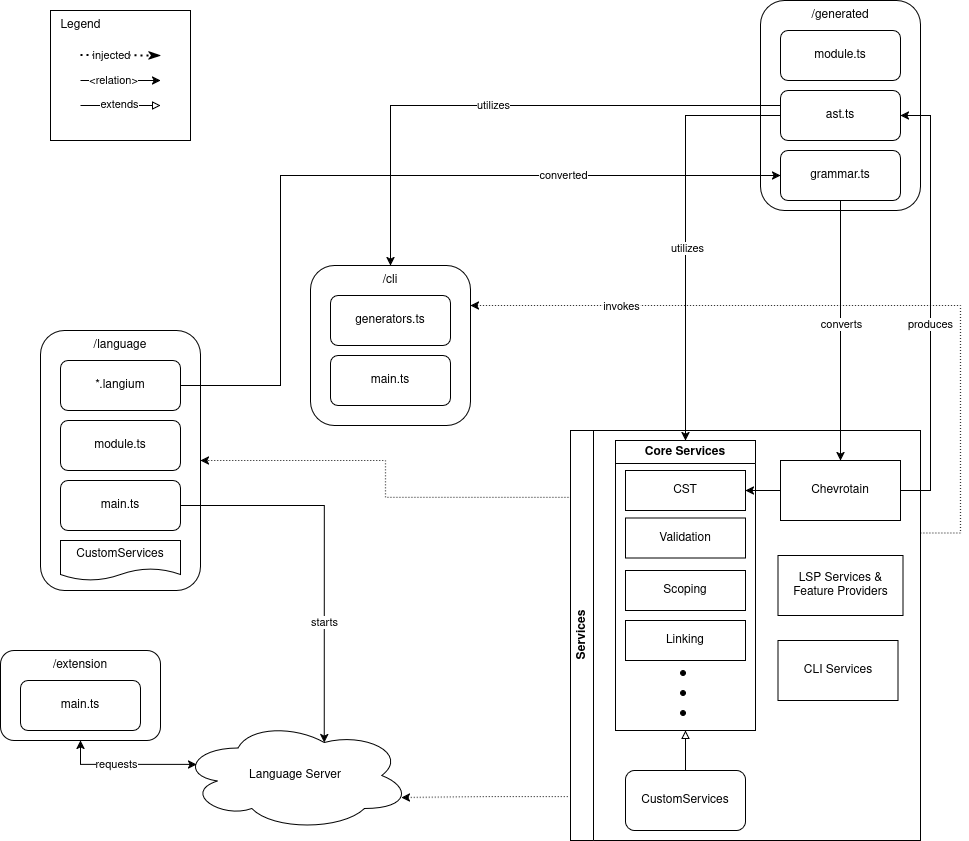
\includegraphics[width=\textwidth]{graphics/langiumArchitecture.png}
  \caption{Architecture overview of a Langium project}
  \label{fig:langium-architecture}
\end{figure}


\section{Module Decomposition}
describe diretories
what do waht do? generators, cli, validation, custom services...

Langium projects can easily be created with the support of the scaffolding tool \verb|Yeoman|, producing a structured mock project including a sample language definition.
Most of the definitions are found in the \verb|src| directory \ref{fig:langium-architecture}, encompassing fnctionality for the Language Server, the extension and actual language tooling.

\begin{description}
  \item[\code{language/}] Assembles the core of any Langium project. It includes the \code{.langium} file, in which the custom language grammar is defined, as well as the code that starts the Language Server with all necessary services bundled.
  \item[\code{cli/}] Provides functionality for CLI interactions, command parsing, and generators. The generators in this folder invoke processes that generate artifacts from the language and input files;
  they are typically used only offline and are called once rather than continuously via the CLI and support efficient pipelining.
  \item[\code{extension/}] Contains the VS Code extension bootstrap code needed to connect to the Language Server and utilize LSP support features. All folders except the CLI/ are bundled into the extension itself.
  \item[\code{generated/}] Contains artifacts produced from the grammar definition in the \code{.langium} file. This includes TypeScript AST type definitions, which are essential for further analysis and validation, as well as the preliminary parsed grammar rules formatted for the Chevrotain engine to generate parsers.
  \item[\textbf{Services}] The Services in Langium are a collection of utility classes and helper functions offered to every component of a language project via dependency injection. They cover an extensive range of functionality, from LSP-specific features - such as providers for context-aware code completion, rich hover tooltips, signature help, go-to-definition and find-references - to core language utilities that expose parsed documents as both AST and CST models, manage workspace state and context information (including indexing, scoping, and name resolution), synchronize the in-memory document model and perform validation checks. Because the parts are wired up as an injectable service, precise consumptions of the capabilities needed is possible. Morover it Langium enables developers to swap in custom implementations to extend the language's behavior. ..expand on CustpmServices
\end{description}


Modules  .... register services, expose interfaces

Although the crucial segments are located inside \code{/src}, files of interest ... Szntax config

syntax TextMate Monarch

Validation.ts  was already placed in /language, subsequenntly, other custom services also implementd here

Lastly, situated at top-level in the \verb|src| directory are three files: \verb|setup....ts| \verb|setup....ts| \verb|setup....ts|, which are invoked
by 

\begin{description}
  \item[\texttt{cli/cli-util.ts}] Shared helper routines for the CLI (file I/O, path resolution, error reporting).
  \item[\texttt{cli/generator.ts}] Yeoman-based scaffolder that bootstraps a new Langium DSL project with templates and example code.
  \item[\texttt{cli/main.ts}] Entry point for the CLI: parses arguments and dispatches subcommands (generate, validate, serve-lsp).
  \item[\texttt{directory.txt}] Snapshot of the directory structure, typically generated by \texttt{tree}, for documentation.
  \item[\texttt{extension/main.ts}] VS Code extension bootstrap: launches the LSP server, sets up the client, handles activation/deactivation.
  \item[\texttt{language/generated/ast.ts}] Auto-generated interfaces for each AST node, defining the DSL’s abstract syntax.
  \item[\texttt{language/generated/grammar.ts}] Auto-generated Chevrotain grammar: token definitions, regex patterns, and rules.
  \item[\texttt{language/generated/module.ts}] DI module binding parser, lexer, CST visitor, and other services into Langium’s registry.
  \item[\texttt{language/hello-world.langium}] The Langium grammar file: terminal and parser rule definitions in Langium DSL.
  \item[\texttt{language/hello-world-module.ts}] Extension of the generated module for custom services (linkers, formatters, completions).
  \item[\texttt{language/hello-world-validator.ts}] Hand-written semantic validation rules (e.g., name collisions, type checks).
  \item[\texttt{language/main-browser.ts}] Browser entry point for embedding the language (e.g., in Monaco), using WebSocket/Worker transport.
  \item[\texttt{language/main.ts}] Node-based language-server entry point: configures FS adapter, instantiates services, starts LSP.
  \item[\texttt{setupCommon.ts}] Registers services common to both Node and browser (grammar access, CST→AST visitor, linking, validation).
  \item[\texttt{setupExtended.ts}] Builds on \texttt{setupCommon} to add IDE features (formatting, folding, hover, semantic tokens).
  \item[\texttt{setupClassic.ts}] Classic Node setup: invokes \texttt{setupExtended}, plugs in Node FS and LSP server, exports startup function.
\end{description}


\section{Data Flow and Control Flow}

\section{Language Server Protocol}
control flow of lsp from file to lsp to editor

custom providers, computators

\chapter{Implementation Details}
\label{sec:langium-grammar}
\section{Langium Grammar Definition for \textit{Miniprob}}
\section{Type System and Semantic Checks}
\section{VS Code Extension Points}
textmate highlighting lang-config.json
\section{Testing \& Validation}

\chapter{Performance \& Usability}
\section{Parsing Speed}
\section{Editor Responsiveness}
\section{User Feedback}